\chapter{แบบฝึกหัดการแนบรูป}
จงใช้โครงร่างของแฟ้มต้นฉบับต่อไปนี้ เติมข้อความระหว่าง \lstinline|\begin{document}| กับ \lstinline|\end{document}| เพื่อสร้างเอกสารผลลัพธ์ดังแสดงในหน้าถัดไป

\begin{lstlisting}
\documentclass[a4paper]{report}

\usepackage[top=2cm, bottom=2cm, left=2cm, right=2cm]{geometry}

\usepackage{fontspec}
\setmainfont[Scale=1.6]{TH Sarabun New}
\XeTeXlinebreaklocale “th”
\XeTeXlinebreakskip = 0pt plus 1pt
\linespread{1.2}

\usepackage{graphicx}
\usepackage{float}
\usepackage{url}

\begin{document}

\end{document}
\end{lstlisting}

สิ่งที่ต้องค้นคว้าเพิ่มเติม
\begin{itemize}
	\item การใช้เชิงอรรถ (footnote)
\end{itemize}

\newpage
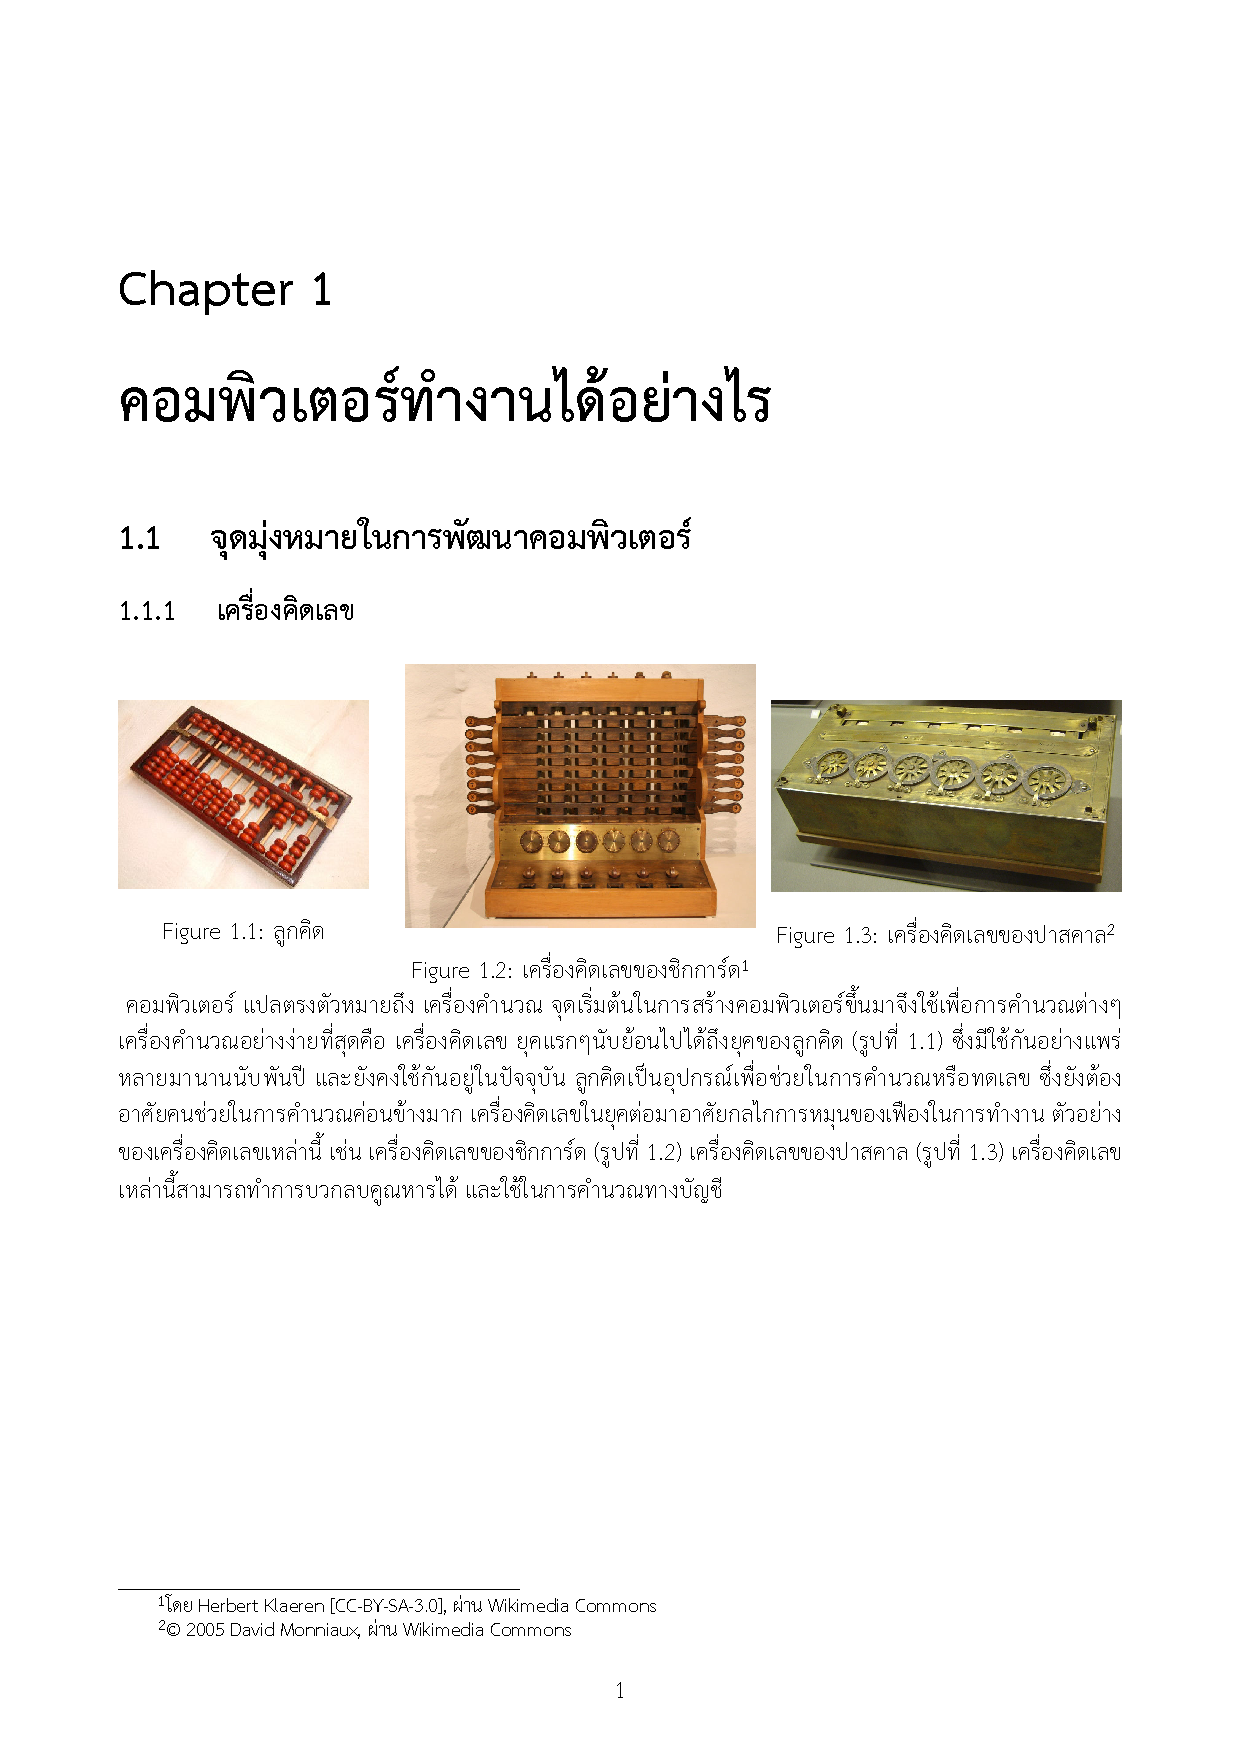
\includepdf{ex1.pdf}
